% !TEX encoding = UTF-8 Unicode
\documentclass[a4paper]{article}
\usepackage{geometry}
 \geometry{
 a4paper,
 total={150mm,240mm},
 left=30mm,
 top=30mm,
 }

\usepackage{color}
\usepackage{url}
\usepackage[T2A]{fontenc} % enable Cyrillic fonts
\usepackage[utf8]{inputenc} % make weird characters work
\usepackage{graphicx}
%\usepackage[]{algorithm2e}
\usepackage{caption}
\usepackage{float}

\usepackage[english,serbian]{babel}
%\usepackage[english,serbianc]{babel} %ukljuciti babel sa ovim opcijama, umesto gornjim, ukoliko se koristi cirilica

\usepackage[unicode]{hyperref}
\hypersetup{colorlinks,citecolor=green,filecolor=green,linkcolor=blue,urlcolor=blue}

\usepackage{listings}

%\newtheorem{primer}{Пример}[section] %ćirilični primer
\newtheorem{primer}{Primer}[section]

\definecolor{mygreen}{rgb}{0,0.6,0}
\definecolor{mygray}{rgb}{0.5,0.5,0.5}
\definecolor{mymauve}{rgb}{0.58,0,0.82}

\lstset{ 
  backgroundcolor=\color{white},   % choose the background color; you must add \usepackage{color} or \usepackage{xcolor}; should come as last argument
  basicstyle=\scriptsize\ttfamily,        % the size of the fonts that are used for the code
  breakatwhitespace=false,         % sets if automatic breaks should only happen at whitespace
  breaklines=true,                 % sets automatic line breaking
  captionpos=b,                    % sets the caption-position to bottom
  commentstyle=\color{mygreen},    % comment style
  deletekeywords={...},            % if you want to delete keywords from the given language
  escapeinside={\%*}{*)},          % if you want to add LaTeX within your code
  extendedchars=true,              % lets you use non-ASCII characters; for 8-bits encodings only, does not work with UTF-8
  firstnumber=1000,                % start line enumeration with line 1000
  frame=single,	                   % adds a frame around the code
  keepspaces=true,                 % keeps spaces in text, useful for keeping indentation of code (possibly needs columns=flexible)
  keywordstyle=\color{blue},       % keyword style
  language=Python,                 % the language of the code
  morekeywords={*,...},            % if you want to add more keywords to the set
  numbers=left,                    % where to put the line-numbers; possible values are (none, left, right)
  numbersep=5pt,                   % how far the line-numbers are from the code
  numberstyle=\tiny\color{mygray}, % the style that is used for the line-numbers
  rulecolor=\color{black},         % if not set, the frame-color may be changed on line-breaks within not-black text (e.g. comments (green here))
  showspaces=false,                % show spaces everywhere adding particular underscores; it overrides 'showstringspaces'
  showstringspaces=false,          % underline spaces within strings only
  showtabs=false,                  % show tabs within strings adding particular underscores
  stepnumber=2,                    % the step between two line-numbers. If it's 1, each line will be numbered
  stringstyle=\color{mymauve},     % string literal style
  tabsize=2,	                   % sets default tabsize to 2 spaces
  title=\lstname                   % show the filename of files included with \lstinputlisting; also try caption instead of title
}

\begin{document}

\title{Fazi neuronska mreža\\ \small{Seminarski rad u okviru kursa\\Računarska inteligencija\\ Matematički fakultet}}

\author{Katarina Savičić, Bojana Ristanović\\ mi16261@alas.matf.bg.ac.rs, mi16045@alas.matf.bg.ac.rs}

\maketitle

\abstract{
U ovom radu će biti predstavljena fazi neuronska mreža. Konkretnije, ovaj metod je korišćen kao metod klasifikacije podataka 
koji u trening fazi koristi min-max algoritam, a u test fazi koristi k najbližih suseda. Nakon opisa algoritma, prikazana je njegova
praktična primena. Na kraju, rezultati su upoređeni sa autorima rada \emph{Understanding Fuzzy Neural Network using code and animation} kao i sa običnim algoritmom KNN (k najbližih suseda).
\\
\\
\textbf{Ključne reči:} fazi logika, neuronske mreže, min-max, knn, klasifikacija.
}
\tableofcontents

\newpage

\section{Uvod}
\label{sec:uvod}

Fazi neuronska mreža (eng. \emph{Fuzzy neural network}) je sistem za učenje koji pronalazi parametre fazi sistema koristeći tehnike aproksimacije neuronskih mreža. To je hibridni inteligentni sistem koji kombinuje tehnike rasuđivanja fazi logike sa tehnikama učenja neuronskih mreža.\cite{fnn}

Fazi min-max klasfikator (eng. \emph{The fuzzy min–max (FMM)}) je sistem koji formira hiperboksove za klasifikaciju i predviđanje. U ovom radu je pokušana modifikacija FMM-a korišćenjem algoritma k najbližih suseda (eng. \emph{k-nearest neighbors algorithm (k-NN)}) u procesu predviđanja klasa prosleđenih podataka.

\section{Fazi logika}
\label{sec:fazilogika}

Kod klasične logike, promenljive mogu uzeti jedino vrednosti 1 ili 0 (tačno ili netačno). Kod fazi logike se skup vrednosti proširuje, pri čemu 
se dozvoljava da promenljive mogu uzeti realne vrednosti unutar nekog intervala. Drugim rečima, pretpostavlja se da ne mora sve biti u 
potpunosti istinito ili u potpunosti neistinito, već se dozvoljava određen nivo delimične istine. Na primer, za nešto možemo reći da je 
najverovatnije istina, pa odgovarajuća promenljiva može imati vrednost 0.9, a u nešto drugo možemo imati veliku sumnju, ali ostavljati 
malu verovatnoću da bude istinito, pa odgovarajuća logička promenljiva tada može imati vrednost 0.1. \cite{fl}

Da li nešto pripada skupu možemo odrediti pomoću funkcije pripadnosti. Ona kod klasične logike ima vrednost 0 ili 1, zato što nešto može 
ili ne da pripada skupu. Kod fazi logike ova funkcija ima vrednost između 0 i 1. \cite{fl}


\section{Neuronske Mreže}
\label{sec:neuronskemreze}

U istraživanju podataka veštačke neuronske mreže su familija statističkih modela učenja inspirisana biološkim neuronskim mrežama. 
Koriste se u svrhu aproksimacije funkcija koje mogu zavisiti od velike količine ulaznih podataka, a koje su u principu nepoznate. Veštačke 
neuronske mreže su sistemi međusobno povezanih neurona, koji šalju poruke jedni drugima. Veze između ovih neurona imaju numeričke 
težine koje mogu biti podložne promenama u zavisnosti od iskustva, što neuronske mreže čini adaptivnim i sposobnim za učenje. Osnovna 
ideja veštačke neuronske mreže je simulacija velike količine gusto napakovanih, međusobno povezanih nervih ćelija u okviru 
računara, tako da je omogućeno učenje pojmova, prepoznavanje šablona i donošenje odluka na način koji je sličan čovekovom.
Neuronska mreža se ne programira eksplicitno da uči, ona to radi sama, isto kao i mozak.\cite{master_rad}

Tipična neuronska mreža ima od nekolicine do stotinu, hiljadu, ili pak milion veštačkih neurona tj. jedinica, umreženih u serije slojeva, gde 
je svaki neuron povezan sa oba sloja sa obe strane. Neki od njih, koji se nalaze u početnom sloju, tj. sloju ulaza, dizajnirani su tako da
dobijaju različite oblike informacija iz spoljašnjeg sveta. Jedinice koje se nalaze na suprotnoj strani mreže, u krajnjem sloju, tj. sloju izlaza, 
signaliziraju način na koji mreža reaguje na naučene informacije. Između leži jedan ili više skrivenih slojeva, koji zajedno čine većinu
veštačkog mozga.\cite{master_rad}

\section{K najbližih suseda}
\label{sec:knn}

Algoritam k najbližih suseda je algoritam otkrivanja zakonitosti u podacima koji se koristi za probleme predviđanja ishoda (bilo da je 
numerička ili nenumerička vrednost), a na osnovu sličnosti slučaja za koji treba doneti odluku sa slučajevima iz tabele slučajeva (baze
znanja). Kada je potrebno doneti odluku posmatra se k najbližih (najsličnijih) suseda i donosi se
ona odluka koja se najčešže pojavljivala kod posmatranih k najbližih suseda.

Izbor parametra k je izuzetno važan i kompleksan korak. Ukoliko izaberemo malu vrednost k, onda možemo doći do situacije da nam
šum u podacima (npr. pogrešno doneta odluka) utiče na dalje odluke. Ako izaberemo preveliko k, onda nam slučajevi koji nisu slični slučaju 
za koji se predviđa ishod utiču na odluku.\cite{knn}

\section{Fazi min-max klasifikator (FMM)}
\label{faziminmaxcl}

Osnovna ideja je da se na osnovu funkcije pripadnosti koja se koristi u Fazi logici može odrediti kojoj klasi pripada instanca koju 
klasifikujemo. U ovom slučaju instanca je uređeni par realnih brojeva, koji se može predstaviti kao tačka u koordinatnom sistemu. 
Klasa instance će biti ona za koju funkcija pripadnosti daje najveću vrednost. Postavlja se pitanje kako predstaviti fazi skup?\cite{mmf}

\subsection{Hiperboks  (eng. \emph{Hyperbox})}
\label{hiperboks}

Fazi skup možemo definisati kao pravougaonik čije dužine stranica mogu uzimati vrednost od 0 do 1. Ovaj skup je takav da ako se tačka 
nalazi unutar pravouganika, vrednost njene funkcije pripadnosti je 1. Pravougaonik je definisan svojom najmanjom (donjom levom) i 
najvećom (gornjom desnom) tačkom. Te tačke ćemo označiti redom slovima v i w.

Vrednost funkcije pripadnosti za svaku tačku koja je van pravougaonika se smanjuje sa povećanjem udaljenosti tačke od pravougaonika. 
Formula za računanje funkcije pripadnosti nekom pravougaoniku, tj. fazi skupu, je data u nastavku:

\begin{equation}
    b_j(A_h) = \frac{1}{2n}\sum_{i=1}^{n}[max(0, 1 - max(0, \gamma min(1, a_{hi}-w_{ji}))) + max(0, 1 - max(0, \gamma min(1, v_{ji}-a_{hi})))]
\end{equation}

$A_h$ obrazac za koji računamo funkciju pripadnosti, $b_j$ fazi skup a $n$ dimenzija (u našem slučaju 2). $\gamma$ je hiperparametar 
koji se naziva osetljivost ili stopa smanjenja i može se koristiti za kontrolisanje vrednosti funkcije pripadnosti.

Kod neuronske mreže imamo prvi sloj koji predstavlja ulazne čvorove za podatke. Sledeći sloj su čvorovi koji predstavljaju hiperbokseve, tj. 
svaki čvor predtavlja jedan hiperboks koji pripada nekoj klasi i definisan je dvema tačkama. Hiperboks je prethodno pomenuti 
pravougaonik. Poslednji sloj čvorova predstavlja izlaz, odnosno klasu. U poslednjem sloju može biti više čvorova, u zavisnosti od broja 
postojećih klasa. Kada gledamo vrednost klase, svaki čvor koji predtavlja klasu definisan je njavećom vrednošću funkcije pripadnosti od 
svih funkcija pripadnosti računate za sve hiperbokseve koje pripadaju datoj klasi. Dakle, svaka klasa može imati jedan ili više hiperbokseva, 
vrednost u čovoru je maksimalna vrednost funkcije pripadnosti razmatranog podatka tim hiperboksevima. Na kraju se porede vrednosti u 
svim čvorovima koji predtavljaju klase i bira se klasa koja ima najveću vrdnost. \cite{mmf}

\subsection{Algoritam}
\label{algoritam}

Kako bismo sproveli pomenuti način klasifikacije, potrebno je da definišemo hiperbokseve za sve klase. To ćemo uraditi na osnovu skupa za 
treniranje, odnosno istreniraćemo klasifikator tako što ćemo napraviti hiperbokseve za postojeće klase. Algoritam se sastoji iz dve faze: 
proširenja i kontrakcije. \cite{mmf}

\subsubsection{Faza proširenja}
\label{prosirenje}

Imamo instancu $X_h$ iz trening skupa, koja pripada klasi $Y$. Prvo proverimo sve hiperbokseve koji pripadaju klasi Y i računamo funkciju 
pripadnosti za svaki. Hiperboks sa najvećom funkcijom pripadnosti je najpogodniji za proširenje. Neka $B_j$ bude jedan takav hiperboks. 
Pre nego što ga proširimo računamo kriterijum ekspaztije dat sledećom formulom:

\begin{equation}
    n\theta >= \sum_{i=1}^{n}(max(w_{ji}, x_{hi}) - min(v_{ji}, x_{hi}))
\end{equation}

gde je $\theta$ hiper parametar koji predstavlja kriterjum proširenja i kontroliše maksimalno proširenje dozvoljeno za hiperboks. Ako 
zadovoljava kriterijum, hiperboks se širi na sledeći način:

\begin{equation}
    v_{ji}^{new} = min(v_{ji}^{old}, x_{hi})
    w_{ji}^{new} = min(w_{ji}^{old}, x_{hi})
\end{equation}

gde su v i w minimalna i maksimalna tačka hiperboksa. Hiperboks se čiri tako da je $X_h$ uključena u region.

Ukoliko kriterijum širenja nije zadovoljen, pravi se novi hiperboks za klasu $Y$, takav da su mu minimalna i maksimalna tačka jednake i 
imaju vrednost $X_h$. Kada proširimo hiperboks, može doći do preklapanja sa drugim hiperboksom. Ovo nije toliko problem ako je u 
pitanju hiperboks iz iste klase, ali jeste ukoliko je u pitanju hiperboks koji pripada nekoj drugoj kasi. Zbog toga imamo fazu kontrakcije.\cite{mmf}

\subsubsection{Faza kontrakcije}
\label{kontrakcija}

Pronašli smo hiperboks koji smo proširili i sada treba da proverimo da li postoji preklapanje sa drugim hiperboksom. Dozvoljeno je 
preklapanje izmedju iperbokseva iste klase, pa treba samo da proverimo za hiperbokseve drugih klasa.

Proveru da li postoji preklapnje vršimo preko tačaka koje odredjuju hiperbokseve. Gledamo po svim dimenzijama da li postoji preklapanje i 
beležimo rezultate. Onda tražimo dimenziju po kojoj je preklapanje najmanje. Slučajevi koji pokrivaju proveru proveru preklapanja su dati u 
kodu. Kada nađemo dimenziju po kojoj je preklapanje minimalo, hoćemo da smanjimo hiperboks po toj dimenziji. Slučajevi koji pokrivaju 
način smanjenja hiperboksa takođe se nalaze u kodu i neće biti predstavljeni ovde.

Poenta celog algoritma je naći odgovarajući hiperboks, proširiti ga ako je to moguće, ako ne naći drugi koji je moguće proširiti, ili dodati 
novi, proveriti da li postoji preklapanje i izvršiti kontrakciju ukoliko postoji. \cite{mmf}

\subsection{Modifikacije algoritma}

U originalnom algoritmu se za određivanje klase uzima samo najveća vrednost klase, koja predstavlja najveću vrednost funkcije pripadnosti 
za hiperbokseve te klase. Mi smo algoritam izmenili tako da ne gleda jednu najveću vrednost već uzima u obzir nekoliko vrednosti.
Umesto da gledamo funkcije pripadnosti i tražimo najveće vrdnosti, gledali smo rastojanje svake tačke od hiperboksa i tražili najmanje 
rastojanje. Pretpostavili smo da rastojanje od hiperboksa možemo posmatrati kao rastojanje od prave koja prolazi kroz tačke koje određuju 
hiperboks. Sortirali smo rastojanja od svih hiperbokseva rastuće i primenili metod k najbližih suseda. Metod smo primenili tako što smo 
uzeli k najmanjih rastojanja, gledali kojim klasama pripadaju hiperboksevi i kao klasu instance uzeli najbrojniju klasu među 
hiperboksevima.


\section{Rezultati}
\label{sec:rezultati}

Za testiranje rezultata korišćena su dva skupa podataka. Prvi je iris 
skup koji se sastoji od 3 vrste cveta Iris - Setosa, Versicolour, Virginica. 
Sadrži 150 instanci i ima 5 atributa koji predstavljaju dužinu i širinu latica 
(eng. \emph{petal length, petal width}), dužinu čašičnog listića (eng. \emph{sepal length, sepal width}) i 
vrstu kojoj cvet pripada (eng. \emph{species}). Pošto je algoritam napisan tako da radi za dvodimenzionalne 
ulazne podatke,  izabrali smo 2 atributa: dužinu latica i dužinu čašičnog lista. Podaci su normalizoavni tako da uzimaju 
vrednosti od 0 do 1.

Pokrenut je originalni algoritam sa kriterijumom proširenja 0.4, modifikovani algoritam sa istim kriterijumom i 4 najbliža suseda kao i 
algoritam KNN za 4 najbliža suseda. Na slici \ref{iris} vidimo da su najbolji rezltati dobije algoritmom KNN. Rezultati prva dva algoritma 
se mogu promeniti sa promenom kriterijuma proširenja. Treba biti oprezan sa postavljanjem ovog kriterijuma jer on utiče na veličinu i na 
broj hiperbokseva, nije poželjno da imamo mnogo malih, kao ni malo velikih hiperbokseva. 

\begin{figure}[h!]
\centering
\captionsetup{justification=centering,margin=2cm}
\begin{center}
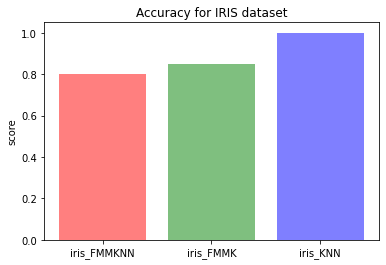
\includegraphics[scale=0.5]{img/iris.png}
\end{center}
\caption{Preciznost na podacima skupa Iris}
\label{iris}
\end{figure}

Wine skup podataka je takođe provučen kroz sva tri algoritma radi poređenja rezultata. Na slici \ref{wine} možemo videti
da algoritam FMM daje najbolje rezultate. Modifikovani KNN algoritam je pogodio klasu za 50\% instanci, međutim preciznost 
ovog algoritma dosta zavisi od prosleđenih parametara tj. od kriterijuma kontrakcije i od broj suseda koji se razmatraju.

\begin{figure}[h!]
\centering
\captionsetup{justification=centering,margin=2cm}
\begin{center}
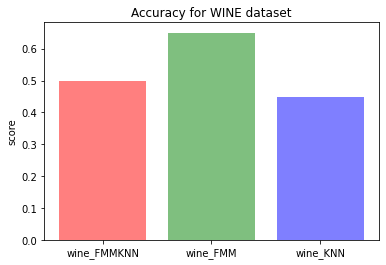
\includegraphics[scale=0.5]{img/wine.png}
\end{center}
\caption{Preciznost na podacima skupa Iris}
\label{wine}
\end{figure}

\section{Zaključak}
\label{sec:zakljucak}

 Hiper parametar $\theta$ se može menjati kako bi se poboljšali rezultati. Ako se koristi visoka vrednost za $\theta$ tada se 
 povećava maksimalna dozvoljena veličina hiperboksa, a to povećava šansu da u tom regionu padne pogrešan uzorak. Sa druge strane, 
 ako se uzme premala vrednost za $\theta$, broj hiperbokseva će se povećavati i preprilagodiće nove tačke. Na ovaj način klasifikator 
 gubi sposobnost dobrog generalizovanja i daje loše performanse. Sa  ovom vrednošću treba eksperimentisati kao bi se pronašla vrednost
 koja daje najbolje performanse.\cite{mmf} Jedno od značajnih poboljšanja algoritma bi bilo njegovo proširenje da radi na više dimenzija.
\addcontentsline{toc}{section}{Literatura}
\appendix
\bibliography{seminarski} 
\bibliographystyle{plain}

\newpage
\appendix

\section{Kod}
\label{kod}

\begin{lstlisting}[caption={Klasa koja predstavlja Fazi Min Max klasifikator koji koristi KNN},frame=single, label=particle]
class FuzzyKNN:
    def __init__(self, sensitivity, exp_bound):
        self.sensitivity = sensitivity
        self.hyperboxes = None
        self.classes = np.array([])
        self.exp_bound = exp_bound
        
    def membership(self, pattern):
        # racuna pripadnost i vraca niz pripadnosti svakom hiperboksu
        min_pts = self.hyperboxes[:, 0, :]
        max_pts = self.hyperboxes[:, 1, :]

        a = np.maximum(0, (1 - np.maximum(0, (self.sensitivity * np.minimum(1, pattern - max_pts)))))
        b = np.maximum(0, (1 - np.maximum(0, (self.sensitivity * np.minimum(1, min_pts - pattern)))))
        
        return np.sum(a + b, axis=1) / (2 * len(pattern))
    
    def overlap_contract(self, index):
        #proveravamo da li se hiperboksevi preklapaju
        contracted = False
        for test_box in range(len(self.hyperboxes)):
            if self.classes[test_box] == self.classes[index]:
                # ignorisemo preklapanje hiperbokseva iste klase
                continue
            expanded_box = self.hyperboxes[index]
            box = self.hyperboxes[test_box]
            
            vj, wj = expanded_box #onaj za koji gledamo da li se preklapa sa nekim
            vk, wk = box

            # moguci slucajevi preklapanja
            # trazimo najmanje preklapanje
            delta_new = delta_old = 1
            min_overlap_index = -1
            for i in range(len(vj)):
                if vj[i] < vk[i] < wj[i] < wk[i]:
                    delta_new = min(delta_old, wj[i] - vk[i])
                elif vk[i] < vj[i] < wk[i] < wj[i]:
                    delta_new = min(delta_old, wk[i] - vj[i])
                
                elif vj[i] < vk[i] < wk[i] < wj[i]:
                    delta_new = min(delta_old, min(wj[i] - vk[i], wk[i] - vj[i]))

                elif vk[i] < vj[i] < wj[i] < wk[i]:
                    delta_new = min(delta_old, min(wj[i] - vk[i], wk[i] - vj[i]))

                if delta_old - delta_new > 0:
                    min_overlap_index = i
                    delta_old = delta_new

            # ako ima preklapanja, 
            # gledamo po kojoj strani smanjujemo hiperbokseve
            if min_overlap_index >= 0:
                i = min_overlap_index
                if vj[i] < vk[i] < wj[i] < wk[i]:
                    vk[i] = wj[i] = (vk[i] + wj[i])/2

                elif vk[i] < vj[i] < wk[i] < wj[i]:
                    vj[i] = wk[i] = (vj[i] + wk[i])/2

                elif vj[i] < vk[i] < wk[i] < wj[i]:
                    if (wj[i] - vk[i]) > (wk[i] - vj[i]):
                        vj[i] = wk[i]

                    else:
                        wj[i] = vk[i]

                elif vk[i] < vj[i] < wj[i] < wk[i]:
                    if (wk[i] - vj[i]) > (wj[i] - vk[i]):
                        vk[i] = wj[i]

                    else:
                        wk[i] = vj[i]

                self.hyperboxes[test_box] = np.array([vk, wk])
                self.hyperboxes[index] = np.array([vj, wj])
                contracted = True
                
        return contracted
    
    def train_pattern(self, X, Y):
        # funkcija koja trenira klasifikator
        target = Y
        
        # ako nemamo tu klasu u klasama
        if target not in self.classes:
            # pravimo hiperboks
            if self.hyperboxes is not None:
                self.hyperboxes = np.vstack((self.hyperboxes, np.array([[X, X]])))
                self.classes = np.hstack((self.classes, np.array([target])))
       
            else:
                self.hyperboxes = np.array([[X, X]])
                self.classes = np.array([target])
        else:

            # sortiramo pripadnosti svim hiperboksevima za trazenu klasu
            memberships = self.membership(X)
            memberships[np.where(self.classes != target)] = 0
            memberships = sorted(list(enumerate(memberships)), key=lambda x: x[1], reverse=True)
            
            # Sirimo hiperboks
            count = 0
            while True:
                index = memberships[count][0]
                min_new = np.minimum(self.hyperboxes[index, 0, :], X)
                max_new = np.maximum(self.hyperboxes[index, 1, :], X)
                
                if self.exp_bound * len(np.unique(self.classes)) >= np.sum(max_new - min_new):
                    self.hyperboxes[index, 0] = min_new
                    self.hyperboxes[index, 1] = max_new
                    break
                else:
                    count += 1

                if count == len(memberships):
                    self.hyperboxes = np.vstack((self.hyperboxes, np.array([[X, X]])))
                    self.classes = np.hstack((self.classes, np.array([target])))
                    index = len(self.hyperboxes) - 1
                    break
                    
            contracted = self.overlap_contract(index)
        
    def fit(self, X, Y):
        for x, y in zip(X, Y):
            self.train_pattern(x, y)

    
    # predvidjamo klasu
    def predict(self, X, k):
        
        #uzimamo tacke koje odredjuju hiperbokseve
        min_pts = self.hyperboxes[:, 0, :]
        max_pts = self.hyperboxes[:, 1, :]
      
        # broj klasa 
        # i niz u kome cemo brojati pojavljivanje svake klase
        n_classes = len(np.unique(self.classes))
        cl = np.zeros(n_classes)
        
        # racunamo udaljenost tacke X od svakog hiperboksa
        # tako sto racunamo udaljenost X od prave koja prolazi kroz tacke koje odredjuju hiperboks
        distance = []
        for i in range(len(min_pts)):
            x1 = min_pts[i][0]
            y1 = min_pts[i][1]
            x2 = max_pts[i][0]
            y2 = max_pts[i][1]
            
            if(x1 == x2 and y1 == y2):
                d = abs(math.sqrt((x1-X[0])**2 + (y1 - X[1])**2))
                distance.append(d)
            elif(x1 == x2):
                d = min(abs(math.sqrt((x1-X[0])**2 + (y1 - X[1])**2)), 
                       abs(math.sqrt((x2-X[0])**2 + (y2 - X[1])**2)))
                distance.append(d)
            elif(y1 == y2):
                d = min(abs(math.sqrt((x1-X[0])**2 + (y1 - X[1])**2)), 
                       abs(math.sqrt((x2-X[0])**2 + (y2 - X[1])**2)))
                distance.append(d)
            else:
                d = abs((y2-y1)*X[0] - (x2-x1)*X[1] + x2*y1 - y2*x1) / math.sqrt((y2-y1)**2 + (x2-x1)**2)
                distance.append(d)

        # sortiramo udaljenosti od najmanje ka najvecoj
        # i uzimamo prvih k najblizih hiperbokseva
        distance = sorted(list(enumerate(distance)), key=lambda x: x[1])
        distance = distance[:k]
        distance_index = []
        for i in range(len(distance)):
            distance_index.append(distance[i][0])
            
        # brojimo pojavljivanje svake klase na osnovu hiperboksa koji joj pripada
        for i in range(len(distance_index)):
            index = distance_index[i]
            _class = self.classes[index]
            cl[_class] += 1
        
        # nalazimo najbrojniju klasu koja je konacna klasa X
        max = 0
        final_class = 0
        for i in range (len(cl)):
            if(cl[i] >= max):
                max = cl[i]
                final_class = i
        
        
        return final_class
       
    # funkcija koja racuna procenat uspesno klasifikovanih instanci
    def score(self, X, Y, k):
        count = 0
        for x, y in zip(X, Y):
            pred = self.predict(x, k)
            if y == pred:
                count += 1
        print(count)
        print(len(Y))
        
        return count / len(Y)

\end{lstlisting}



\end{document}
